% Lecture 2: State Estimation Techniques
\documentclass[aspectratio=169]{beamer}
\usetheme{Madrid}
\usecolortheme{whale}

% Packages
\usepackage{amsmath}
\usepackage{graphicx}
\usepackage{hyperref}
\usepackage{listings}
\usepackage{xcolor}
\usepackage{tikz}
\usepackage{algorithm}
\usepackage{algpseudocode}

% Define colors for syntax highlighting
\definecolor{codegreen}{rgb}{0,0.6,0}
\definecolor{codegray}{rgb}{0.5,0.5,0.5}
\definecolor{codepurple}{rgb}{0.58,0,0.82}
\definecolor{backcolour}{rgb}{0.95,0.95,0.92}

% Configure Python style
\lstdefinestyle{pythonstyle}{
    language=Python,
    basicstyle=\ttfamily\tiny,
    backgroundcolor=\color{backcolour},
    commentstyle=\color{codegreen},
    keywordstyle=\color{blue}\bfseries,
    stringstyle=\color{codepurple},
    breakatwhitespace=false,
    breaklines=true,
    captionpos=b,
    keepspaces=true,
    numbers=left,
    numberstyle=\tiny\color{codegray},
    numbersep=5pt,
    showspaces=false,
    showstringspaces=false,
    showtabs=false,
    tabsize=4,
    frame=single,
    morekeywords={self,def,class,return,import,from,as,with},
    emphstyle={\color{blue}},
    emph={numpy,scipy,np,random,multivariate_normal}
}

\lstset{style=pythonstyle}

% Title Page Info
\title{SES/RAS 598: Space Robotics and AI}
\subtitle{Lecture 2: State Estimation Techniques}
\author{Dr. Jnaneshwar Das}
\institute{Arizona State University \\ School of Earth and Space Exploration}
\date{Spring 2025}

% Reduce main text size by 20%
\AtBeginDocument{\fontsize{8}{10}\selectfont}

% TikZ styles for diagrams with reduced font size
\tikzstyle{block} = [rectangle, draw, fill=blue!20, 
    text width=5em, text centered, rounded corners, minimum height=4em, font=\fontsize{6}{8}\selectfont]
\tikzstyle{line} = [draw, -latex']
\tikzstyle{cloud} = [draw, ellipse, fill=red!20,
    minimum height=2em, font=\fontsize{6}{8}\selectfont]

% Reduce figure font sizes by 30%
\tikzset{
    every node/.style={font=\fontsize{5.6}{7}\selectfont},
    every label/.style={font=\fontsize{5.6}{7}\selectfont},
    every pin/.style={font=\fontsize{5.6}{7}\selectfont}
}

\begin{document}

% Title slide
\begin{frame}
    \titlepage
\end{frame}

% Outline
\begin{frame}{Lecture Outline}
    \tableofcontents
\end{frame}

\section{Kalman Filter Fundamentals}

\begin{frame}{Kalman Filter Overview}
    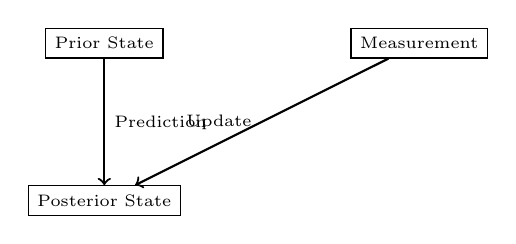
\begin{tikzpicture}
        \node[draw, rectangle] (prior) at (0,0) {Prior State};
        \node[draw, rectangle] (measurement) at (4,0) {Measurement};
        \node[draw, rectangle] (posterior) at (0,-2) {Posterior State};
        
        \draw[->, thick] (prior) -- node[right] {Prediction} (posterior);
        \draw[->, thick] (measurement) -- node[left] {Update} (posterior);
    \end{tikzpicture}
\end{frame}

\begin{frame}{Kalman Filter Steps}
    \begin{columns}[t]
        \column{0.48\textwidth}
        \textbf{Prediction Step}
        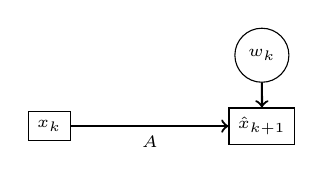
\begin{tikzpicture}[scale=0.9]
            \node[draw, rectangle] (state) at (0,0) {$x_k$};
            \node[draw, rectangle] (predicted) at (3,0) {$\hat{x}_{k+1}$};
            \node[draw, circle] (noise) at (3,1) {$w_k$};
            
            \draw[->, thick] (state) -- node[below] {$A$} (predicted);
            \draw[->, thick] (noise) -- (predicted);
        \end{tikzpicture}
        
        \vspace{0.5cm}
        $\hat{x}_{k+1} = Ax_k + Bu_k$
        \vspace{0.3cm}
        
        $P_{k+1} = AP_kA^T + Q$
        
        \column{0.48\textwidth}
        \textbf{Update Step}
        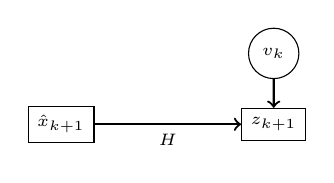
\begin{tikzpicture}[scale=0.9]
            \node[draw, rectangle] (pred) at (0,0) {$\hat{x}_{k+1}$};
            \node[draw, rectangle] (meas) at (3,0) {$z_{k+1}$};
            \node[draw, circle] (noise) at (3,1) {$v_k$};
            
            \draw[->, thick] (pred) -- node[below] {$H$} (meas);
            \draw[->, thick] (noise) -- (meas);
        \end{tikzpicture}
        
        \vspace{0.5cm}
        $K_{k+1} = P_{k+1}H^T(HP_{k+1}H^T + R)^{-1}$
        \vspace{0.3cm}
        
        $x_{k+1} = \hat{x}_{k+1} + K_{k+1}(z_{k+1} - H\hat{x}_{k+1})$
        \vspace{0.3cm}
        
        $P_{k+1} = (I - K_{k+1}H)P_{k+1}$
    \end{columns}
\end{frame}

\begin{frame}[fragile]{Implementation Example: Kalman Filter}
\begin{lstlisting}[language=Python]
import numpy as np

class KalmanFilter:
    def __init__(self, A, B, C, Q, R):
        self.A = A  # State transition matrix
        self.B = B  # Input matrix
        self.C = C  # Measurement matrix
        self.Q = Q  # Process noise covariance
        self.R = R  # Measurement noise covariance
        
    def predict(self, x, P, u=None):
        """Predict next state and covariance."""
        if u is not None:
            x_pred = self.A @ x + self.B @ u
        else:
            x_pred = self.A @ x
        P_pred = self.A @ P @ self.A.T + self.Q
        return x_pred, P_pred
    
    def update(self, x_pred, P_pred, y):
        """Update state estimate using measurement."""
        K = P_pred @ self.C.T @ np.linalg.inv(
            self.C @ P_pred @ self.C.T + self.R)
        x = x_pred + K @ (y - self.C @ x_pred)
        P = (np.eye(len(x)) - K @ self.C) @ P_pred
        return x, P
\end{lstlisting}
\end{frame}

\section{Particle Filters}

\begin{frame}{Introduction to Particle Filters}
    \begin{itemize}
        \item<1-> \textbf{Key Features:}
            \begin{itemize}
                \item Non-parametric estimation
                \item Handles non-linear systems
                \item Represents arbitrary distributions
            \end{itemize}
        \item<2-> \textbf{Working Principle:}
            \begin{itemize}
                \item Particle representation
                \item Sequential importance sampling
                \item Resampling step
            \end{itemize}
        \item<3-> \textbf{Advantages:}
            \begin{itemize}
                \item No linearity assumption
                \item Handles multi-modal distributions
                \item Robust to outliers
            \end{itemize}
    \end{itemize}
\end{frame}

\begin{frame}{Particle Filter Algorithm}
    \begin{algorithm}[H]
    \begin{algorithmic}[1]
        \For{each time step $k$}
            \For{each particle $i$}
                \State Sample new state: $x_k^i \sim p(x_k|x_{k-1}^i, u_k)$
                \State Update weight: $w_k^i = w_{k-1}^i p(z_k|x_k^i)$
            \EndFor
            \State Normalize weights: $w_k^i = w_k^i/\sum_j w_k^j$
            \If{$N_{eff} < N_{threshold}$}
                \State Resample particles
            \EndIf
        \EndFor
    \end{algorithmic}
    \end{algorithm}
\end{frame}

\begin{frame}[fragile]{Implementation Example: Particle Filter}
\begin{lstlisting}[language=Python]
import numpy as np
from scipy.stats import multivariate_normal

class ParticleFilter:
    def __init__(self, n_particles, motion_model, measurement_model):
        self.n_particles = n_particles
        self.motion_model = motion_model
        self.measurement_model = measurement_model
        self.particles = None
        self.weights = None
        
    def initialize(self, initial_state, initial_cov):
        """Initialize particles from Gaussian distribution."""
        self.particles = multivariate_normal.rvs(
            mean=initial_state,
            cov=initial_cov,
            size=self.n_particles
        )
        self.weights = np.ones(self.n_particles) / self.n_particles
        
    def predict(self, u=None):
        """Propagate particles through motion model."""
        for i in range(self.n_particles):
            self.particles[i] = self.motion_model(
                self.particles[i], u)
            
    def update(self, measurement):
        """Update particle weights using measurement."""
        for i in range(self.n_particles):
            likelihood = self.measurement_model(
                measurement, self.particles[i])
            self.weights[i] *= likelihood
        self.weights /= np.sum(self.weights)
        
    def resample(self):
        """Resample particles if effective sample size is low."""
        n_eff = 1.0 / np.sum(self.weights**2)
        if n_eff < self.n_particles / 2:
            indices = np.random.choice(
                self.n_particles,
                size=self.n_particles,
                p=self.weights
            )
            self.particles = self.particles[indices]
            self.weights = np.ones(self.n_particles) / self.n_particles
\end{lstlisting}
\end{frame}

\section{Particle Filter}

\begin{frame}{Particle Filter Overview}
    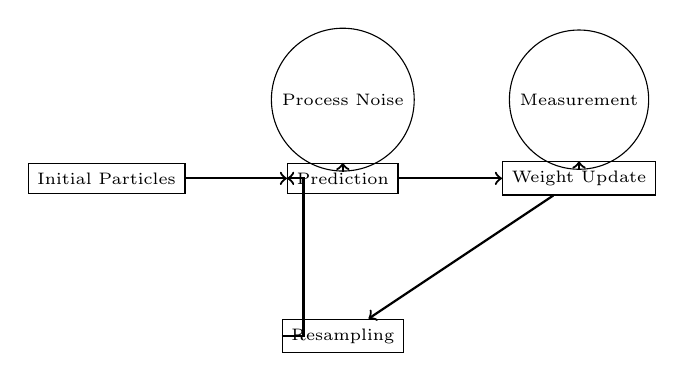
\begin{tikzpicture}
        \node[draw, rectangle] (init) at (0,0) {Initial Particles};
        \node[draw, rectangle] (predict) at (3,0) {Prediction};
        \node[draw, rectangle] (update) at (6,0) {Weight Update};
        \node[draw, rectangle] (resample) at (3,-2) {Resampling};
        \node[draw, circle] (noise) at (3,1) {Process Noise};
        \node[draw, circle] (meas) at (6,1) {Measurement};
        
        \draw[->, thick] (init) -- (predict);
        \draw[->, thick] (predict) -- (update);
        \draw[->, thick] (update) -- (resample);
        \draw[->, thick] (resample) -- ++(-0.5,0) |- (predict);
        \draw[->, thick] (noise) -- (predict);
        \draw[->, thick] (meas) -- (update);
    \end{tikzpicture}
\end{frame}

\begin{frame}{Particle Filter Steps}
    \begin{columns}
        \begin{column}{0.5\textwidth}
            \textbf{Particle Propagation:}
            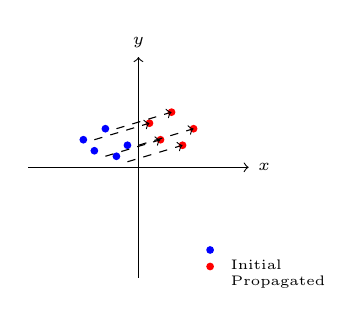
\begin{tikzpicture}[scale=0.7]
                % Draw coordinate system
                \draw[->] (-2,0) -- (2,0) node[right] {$x$};
                \draw[->] (0,-2) -- (0,2) node[above] {$y$};
                
                % Draw initial particles
                \foreach \x/\y in {-1/0.5, -0.8/0.3, -0.6/0.7, -0.4/0.2, -0.2/0.4} {
                    \fill[blue] (\x,\y) circle (2pt);
                }
                
                % Draw propagated particles with noise
                \foreach \x/\y in {0.2/0.8, 0.4/0.5, 0.6/1.0, 0.8/0.4, 1.0/0.7} {
                    \fill[red] (\x,\y) circle (2pt);
                    \draw[->,dashed] (\x-1,\y-0.3) -- (\x,\y);
                }
                
                % Legend
                \node[below right] at (1.5,-1.5) {\tiny Initial};
                \fill[blue] (1.3,-1.5) circle (2pt);
                \node[below right] at (1.5,-1.8) {\tiny Propagated};
                \fill[red] (1.3,-1.8) circle (2pt);
            \end{tikzpicture}
        \end{column}
        
        \begin{column}{0.5\textwidth}
            \textbf{Resampling:}
            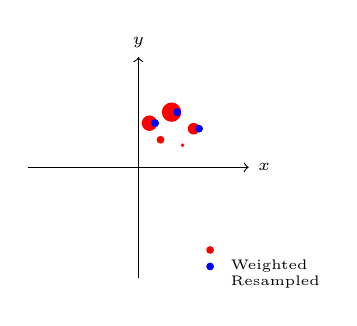
\begin{tikzpicture}[scale=0.7]
                % Draw coordinate system
                \draw[->] (-2,0) -- (2,0) node[right] {$x$};
                \draw[->] (0,-2) -- (0,2) node[above] {$y$};
                
                % Draw weighted particles (size indicates weight)
                \fill[red] (0.2,0.8) circle (4pt);
                \fill[red] (0.4,0.5) circle (2pt);
                \fill[red] (0.6,1.0) circle (5pt);
                \fill[red] (0.8,0.4) circle (1pt);
                \fill[red] (1.0,0.7) circle (3pt);
                
                % Draw resampled particles
                \foreach \x/\y in {0.2/0.8, 0.2/0.8, 0.6/1.0, 0.6/1.0, 1.0/0.7} {
                    \fill[blue] (\x+0.1,\y) circle (2pt);
                }
                
                % Legend
                \node[below right] at (1.5,-1.5) {\tiny Weighted};
                \fill[red] (1.3,-1.5) circle (2pt);
                \node[below right] at (1.5,-1.8) {\tiny Resampled};
                \fill[blue] (1.3,-1.8) circle (2pt);
            \end{tikzpicture}
        \end{column}
    \end{columns}
\end{frame}

\section{Assignment 1: 2D State Estimation}

\begin{frame}{Assignment Overview}
    \begin{itemize}
        \item<1-> \textbf{Objectives:}
            \begin{itemize}
                \item Implement 2D state estimation using ROS2
                \item Compare Kalman and particle filter performance
                \item Visualize results using RViz
            \end{itemize}
        \item<2-> \textbf{Key Components:}
            \begin{itemize}
                \item ROS2 node implementation
                \item Filter implementation
                \item Visualization and analysis
            \end{itemize}
        \item<3-> \textbf{Evaluation:}
            \begin{itemize}
                \item Code quality and documentation
                \item Filter performance metrics
                \item Analysis and discussion
            \end{itemize}
    \end{itemize}
\end{frame}

\begin{frame}[fragile]
\frametitle{ROS2 Environment Setup}
\begin{lstlisting}[language=bash]
# Create ROS2 workspace
mkdir -p ~/ros2_ws/src
cd ~/ros2_ws/src

# Create package
ros2 pkg create --build-type ament_python \
    state_estimation_assignment

# Build workspace
cd ~/ros2_ws
colcon build

# Source workspace
source install/setup.bash
\end{lstlisting}
\end{frame}

\begin{frame}[fragile]
\frametitle{Basic ROS2 Node Structure}
\begin{lstlisting}
import rclpy
from rclpy.node import Node
from geometry_msgs.msg import PoseStamped
from nav_msgs.msg import Odometry

class StateEstimator(Node):
    def __init__(self):
        super().__init__('state_estimator')
        self.subscription = self.create_subscription(
            Odometry,
            'odom',
            self.odom_callback,
            10)
        self.publisher = self.create_publisher(
            PoseStamped,
            'estimated_pose',
            10)
            
    def odom_callback(self, msg):
        # Implement state estimation here
        pass
\end{lstlisting}
\end{frame}

\section{Next Steps}

\begin{frame}{Preparation for Next Week}
    \begin{itemize}
        \item<1-> \textbf{Assignment 1:}
            \begin{itemize}
                \item Review ROS2 basics
                \item Study filter implementations
                \item Start coding basic structure
            \end{itemize}
        \item<2-> \textbf{Reading:}
            \begin{itemize}
                \item Extended Kalman Filter
                \item Unscented Kalman Filter
                \item Advanced particle filter topics
            \end{itemize}
        \item<3-> \textbf{Tools:}
            \begin{itemize}
                \item Test ROS2 installation
                \item Practice with RViz
                \item Explore sensor fusion tutorial
            \end{itemize}
    \end{itemize}
\end{frame}

\begin{frame}{Questions?}
    \begin{center}
        \Huge Thank you!
        
        \vspace{1cm}
        \normalsize
        Contact: jdas5@asu.edu
    \end{center}
\end{frame}

\begin{frame}{Filter Performance Comparison}
    \begin{columns}
        \begin{column}{0.5\textwidth}
            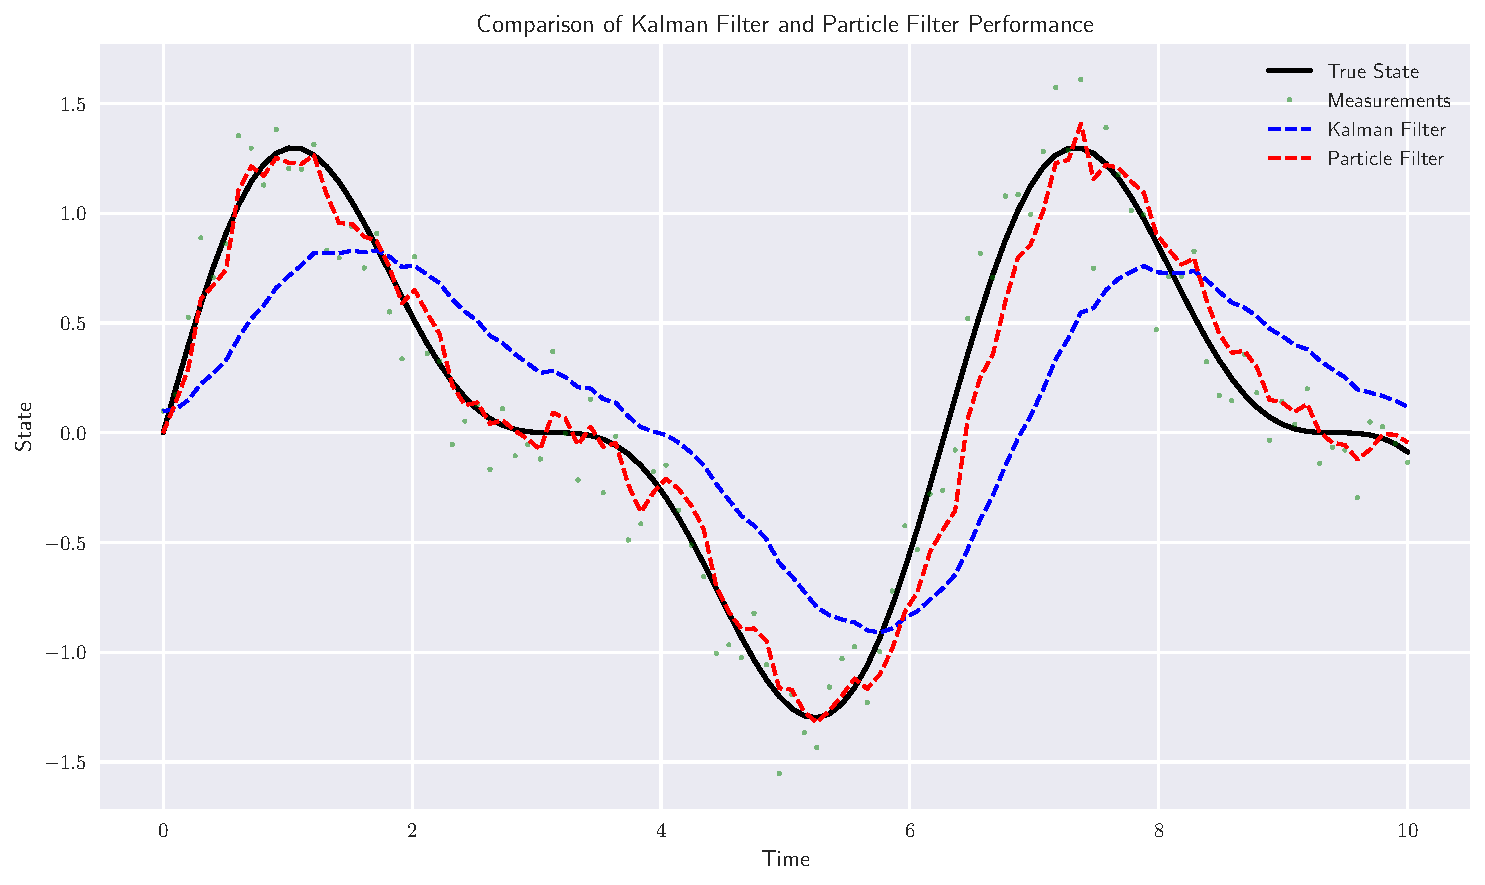
\includegraphics[width=\textwidth]{filter_comparison.pdf}
        \end{column}
        \begin{column}{0.5\textwidth}
            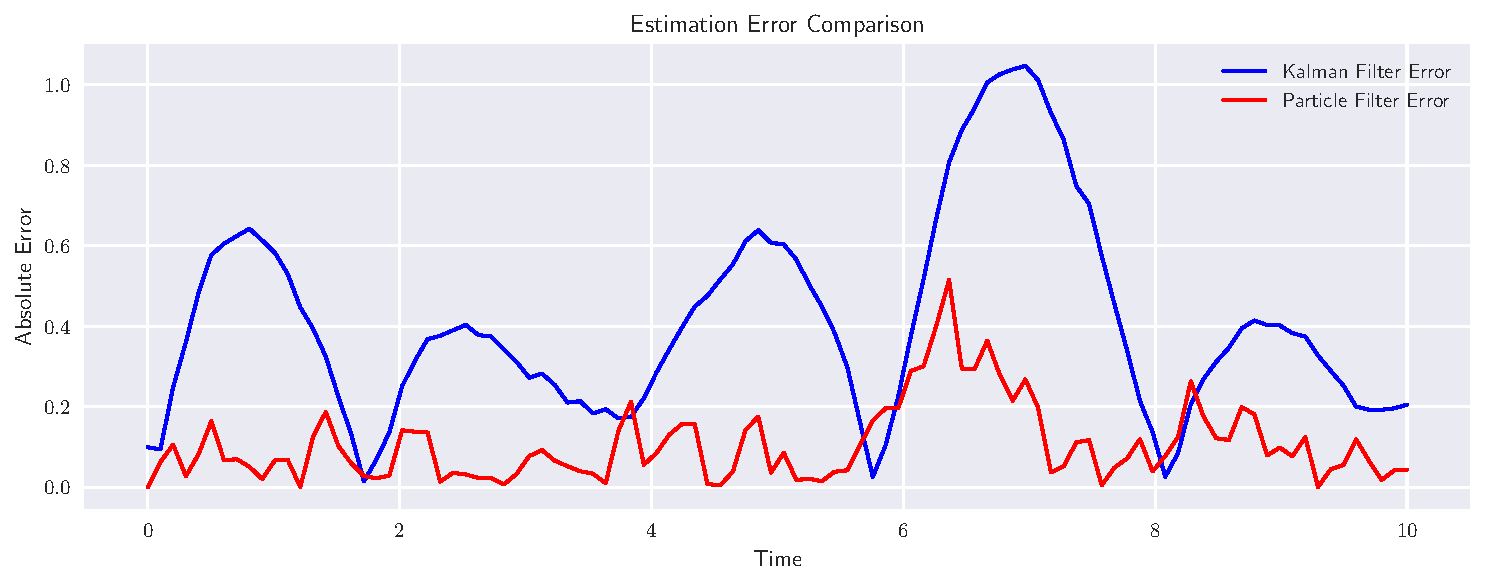
\includegraphics[width=\textwidth]{error_comparison.pdf}
        \end{column}
    \end{columns}
    \vspace{0.3cm}
    \begin{itemize}
        \item Kalman Filter: Optimal for linear systems with Gaussian noise
        \item Particle Filter: Better handles non-linear dynamics and non-Gaussian noise
        \item Trade-off between computational cost and estimation accuracy
    \end{itemize}
\end{frame}

\end{document} 